\subsection{Open-ended task space: XLand 2.0} \label{sec:methods_xverse}

In order to demonstrate fast adaptation across an open-ended task space, we extend the procedurally-generated 3D environment XLand \citep{xland}, which we refer to here as XLand 1.0. In XLand, a task consists of a game, a world, and a list of co-player policies (if any). The game consists of a goal per player, defined as a boolean function (predicate) on the environment state. An agent receives reward if and only if the goal is satisfied. Goals are defined in a synthetic language, and the agent receives an encoding. The world specifies a static floor topology, objects the player can interact with, and spawn locations for players. The agent observes the world, and any co-players therein, via a first-person pixel observation. All fundamental details of the game, world and co-player system are inherited from the original XLand; see~\cite{xland} for a full description and Appendix~\ref{app:xland_changes} for details of the new features we added.

XLand 2.0 extends XLand 1.0 with a system called \textit{production rules}. Each production rule expresses an additional environment dynamic, leading to a much richer and more diverse array of different transition functions than in XLand 1.0. The production rules system can be thought of as a domain-specific language (DSL) to express this diverse array of dynamics. Each production rule consists of:
\begin{enumerate}
    \item A \texttt{condition}, which is a predicate, for example \texttt{near(yellow sphere,black cube)},
    \item A (possibly empty) list of \texttt{spawn}s, which are objects, like \texttt{purple cube, black cube}.
\end{enumerate}

\begin{figure}[t!]
    \centering
    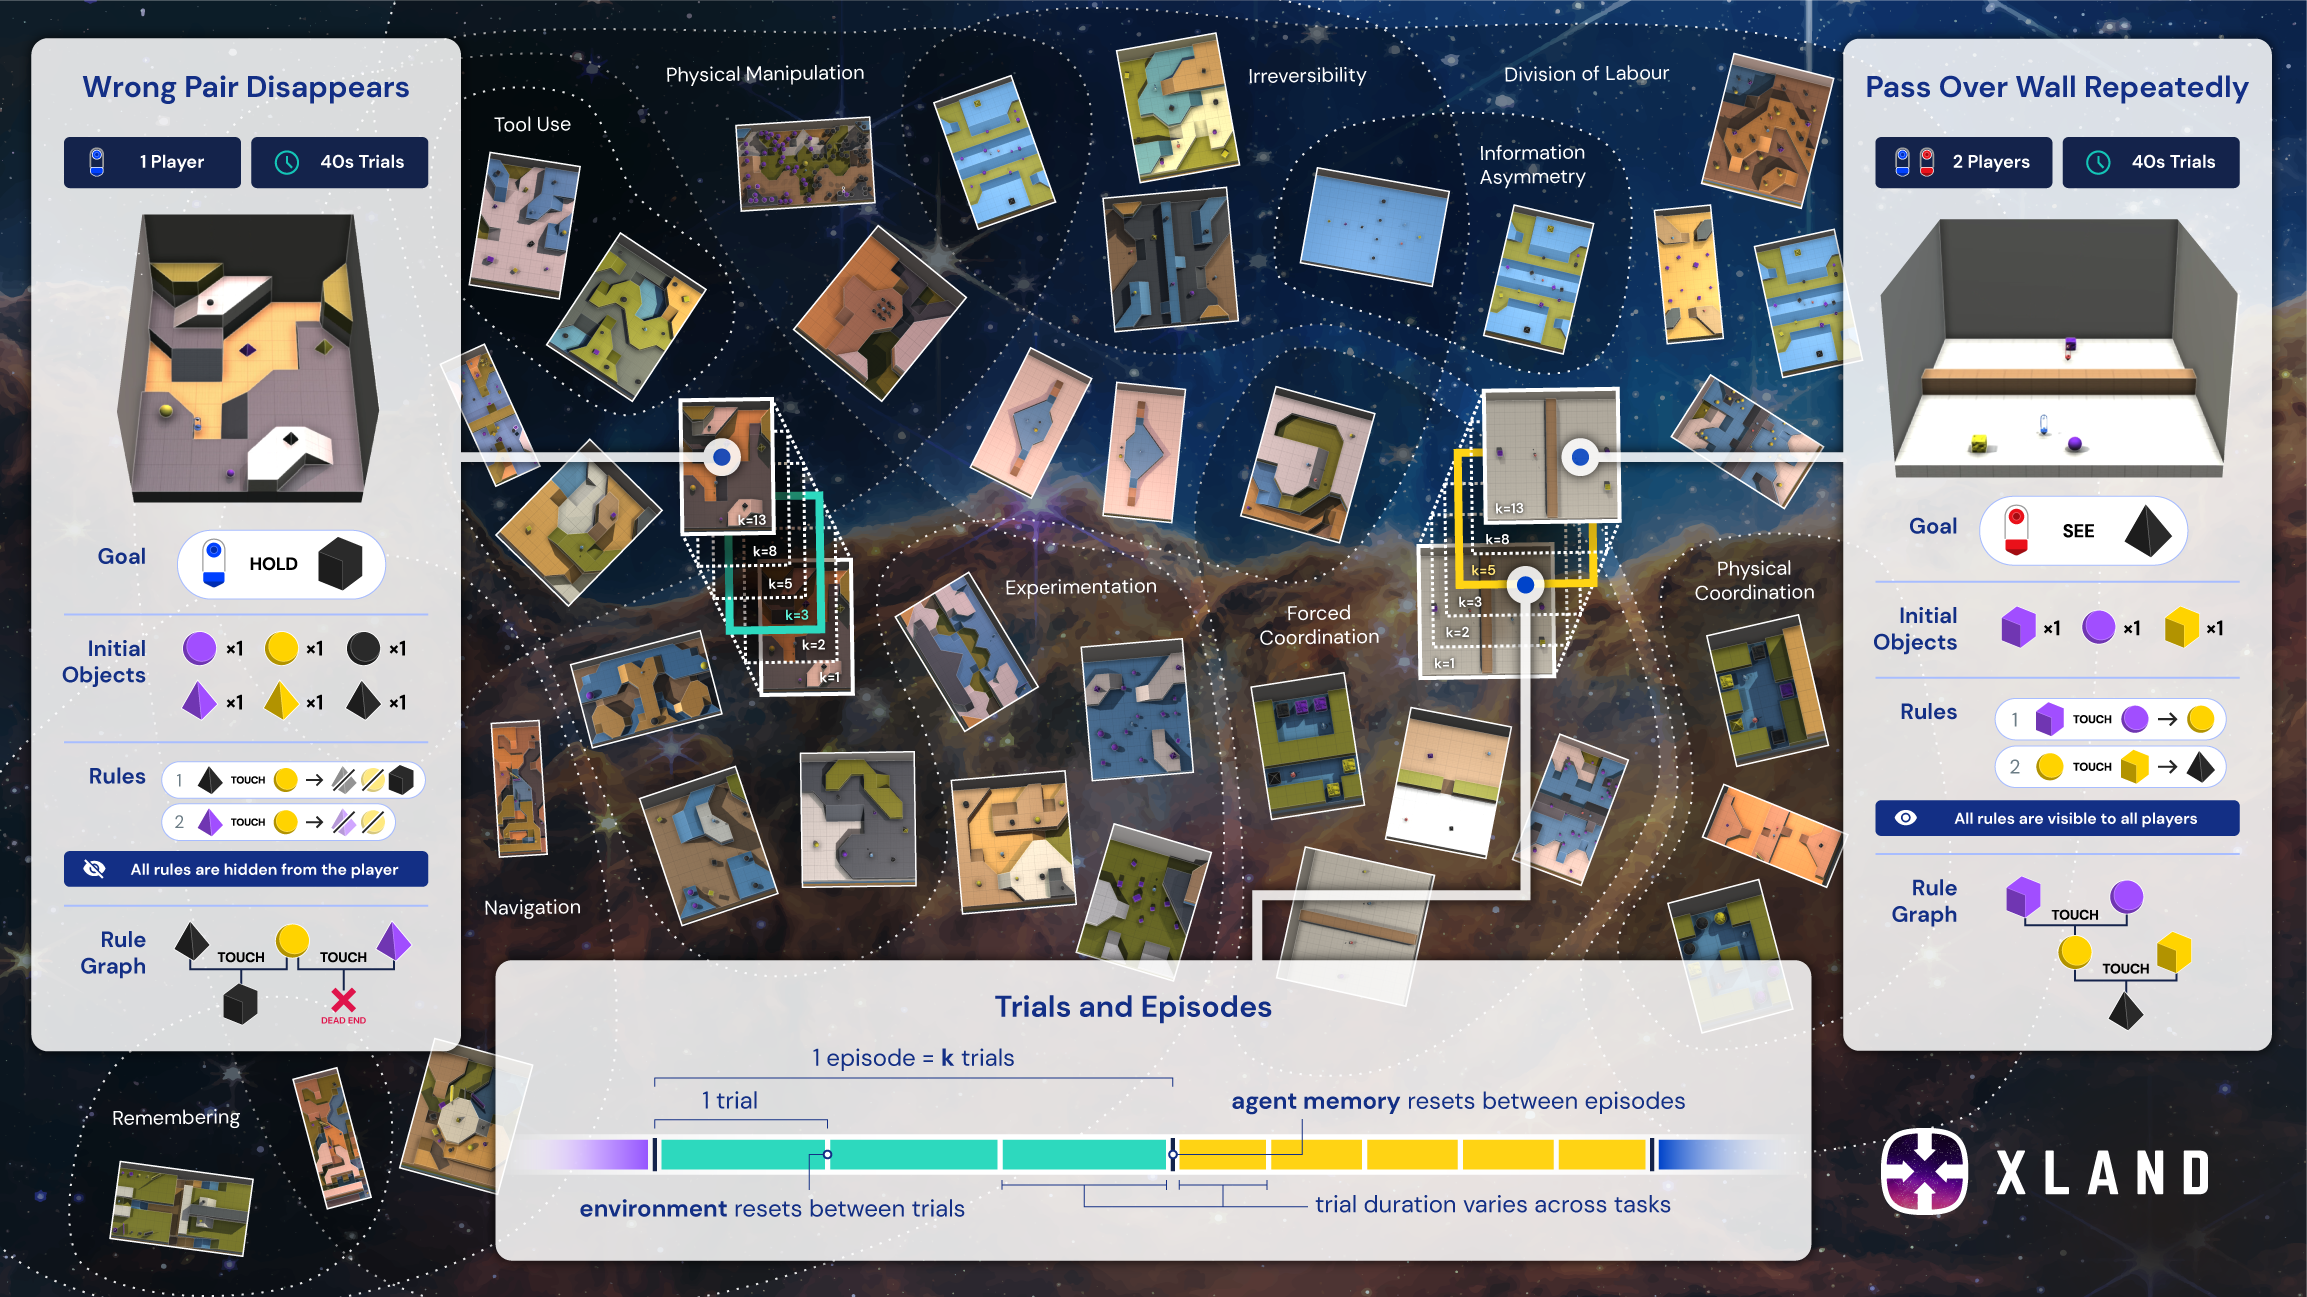
\includegraphics[width=\linewidth]{figures/ada_paper_task_diagram.png}
    \caption{\textbf{XLand 2.0: a vast, smooth and diverse task space of adaptation problems.} Different tasks have different adaptation requirements, such as experimentation, tool use or division of labour. For instance, in a task requiring experimentation, a player might be required to identify which objects can usefully combine, avoiding dead-ends, and then optimise the way in which they combine objects, like a toy version of experimental chemistry. Each task can be run for one or more trials, where the environment is reset between trials, but agent memory is not. Highlighted are two example tasks, \texttt{Wrong Pair Disappears} and \texttt{Pass Over Wall Repeatedly}, showing the goal, initial objects, production rules (``rules'' in the figure) and how agents need to interact with them to solve the task. For full task descriptions see Appendix \ref{appendix:probe_tasks}.}
    \label{fig:xland-overview}
\end{figure}



When \texttt{condition} is satisfied, the objects present in \texttt{condition} get removed from the environment, and the ones in \texttt{spawns} appear.
Each game can have multiple production rules. Production rules can be observable to players, or partially or fully masked, depending on the task configuration. More precisely, there are three distinct mechanisms for hiding production rule information from the players: 

\begin{enumerate}
    \item Hiding a full production rule, where the player only gets information that a rule exists, but neither knows the condition nor what spawns.
    \item Hiding an object, where a particular object is hidden from all production rules. The hidden objects are numbered such that if multiple objects are hidden, the agent can distinguish them.
    \item Hiding a condition's predicate, where the agent gets to know the objects that need to satisfy \textit{some} predicate, but it does not know which one. The hidden predicates are also numbered.
\end{enumerate}

Instead of procedurally generating tasks on the fly, we pre-sample a large pool of tasks. For more details about the specific mechanism we use for pre-sampling tasks, see Appendix \ref{app:presample_tasks}. We visualise the XLand 2.0 task space in Figure \ref{fig:xland-overview}.

